% \input{"IAB/latex/TeX-Folienformat.tex"}
\input{"/Users/jonathanlatner/Google Drive/My Drive/IAB/latex/TeX-Folienformat.tex"}

\documentclass[t,8pt,utfx8]{beamer}
\usepackage{booktabs}
\usepackage{setspace}
\usepackage{parskip}
\usepackage{graphicx}
\usepackage{subcaption}
\setbeamertemplate{caption}[numbered]
\newcommand{\sprache}{\englisch}
\renewcommand{\thesubsection}{\alph{subsection})}
\usepackage[cal=pxtx, scr=dutchcal]{mathalpha}
\usepackage{forest}



\definecolor{codegreen}{rgb}{0,0.6,0}
\definecolor{codegray}{rgb}{0.5,0.5,0.5}
\definecolor{codepurple}{rgb}{0.58,0,0.82}
\definecolor{backcolour}{rgb}{0.95,0.95,0.92}


\usepackage{listings}

% Define style for R code
\lstset{
  language=R,
  basicstyle=\ttfamily\small,
  keywordstyle=\color{blue},
  stringstyle=\color{red},
  commentstyle=\color{green},
  showstringspaces=false,
  numbers=left,
  numberstyle=\tiny\color{gray},
  stepnumber=1,
  numbersep=5pt,
  breaklines=true,
  frame=single
}

\newcommand{\btVFill}{\vskip0pt plus 1filll}


\title{Buyer Beware: Understanding the trade-off between utility and risk in CART based models using simulation data}

\subtitle{
UNECE Expert Meeting on Statistical Data Collection 2025, \newline Barcelona, \newline 15-17. October, 2025}

\author{Jonathan Latner, PhD \newline Dr. Marcel Neunhoeffer \newline Prof. Dr. Jörg Drechsler}

\newcounter{noauthorlines}
\setcounter{noauthorlines}{2} % Wert für 2 Autoren über 2 Zeilen. Ggf. anpassen

% %%%%%%%%%%%%%%
% Ende Anpassung
% %%%%%%%%%%%%%%

% \input{"IAB/latex/TeX-Folienformatierung_CD_2019"}
\input{"/Users/jonathanlatner/Google Drive/My Drive/IAB/latex/TeX-Folienformatierung_CD_2019"}

% Modify the section in toc template to enumerate
\setbeamertemplate{section in toc}{%
    \inserttocsectionnumber.~\inserttocsection\par
}

% use for subsections
% \setbeamertemplate{subsection in toc}{}
\setbeamertemplate{subsection in toc}{%
    \setlength{\parskip}{1mm}
        \hskip2mm -- \hskip1mm\inserttocsubsection\par
}


\usepackage{colortbl}
\definecolor{lightgray}{gray}{0.9}

\usepackage{listings} %include R code
\lstdefinestyle{mystyle}{
    backgroundcolor=\color{backcolour},   
    commentstyle=\color{codegreen},
    keywordstyle=\color{magenta},
    numberstyle=\tiny\color{codegray},
    stringstyle=\color{codepurple},
    basicstyle=\ttfamily\tiny,
    breakatwhitespace=false,         
    breaklines=true,                 
    captionpos=b,                    
    keepspaces=true,                 
    numbers=left,                    
    numbersep=5pt,                  
    showspaces=false,                
    showstringspaces=false,
    showtabs=false,                 
    columns=fullflexible,
    frame=single,
    tabsize=2
}
\lstset{style=mystyle}


\begin{document}


\frame[plain]{\titlepage}

\begin{spacing}{1.25}

%%%%%%%%%%%%%%%%%%%%%%%%%%%%%%%%%%%%%%%%
%%%%%%%%%%%%%%%%%%%%%%%%%%%%%%%%%%%%%%%%
\section{Introduction}\label{sec:introduction}
%%%%%%%%%%%%%%%%%%%%%%%%%%%%%%%%%%%%%%%%
%%%%%%%%%%%%%%%%%%%%%%%%%%%%%%%%%%%%%%%%

\begin{frame}[c,plain]
\vskip-4mm
\begin{beamercolorbox}[wd=\boxwidth,ht=22.11mm]{transparent}%
    \vfill%
    \usebeamerfont{title}%
    \leftinsert%
    \MakeUppercase{Section \ref{sec:introduction}: Introduction
} % <- Hier die Überschrift eintragen
\end{beamercolorbox}
\vskip-3mm
\pgfuseimage{rahmenlinie}
\end{frame}

\begin{frame}{Research Question and Approach}
\begin{itemize}
    \item Research Question: 
    \begin{itemize}
        \item  Do common privacy measures accurately capture disclosure risk in synthetic data generated by CART models?
    \end{itemize}
    \item Context:
    \begin{itemize}
        \item Synthetic data increasingly used to share data while preserving privacy.
        \item CART-based SDGs: high statistical utility, relatively low privacy risk.
    \end{itemize}
    \item Privacy Measures Evaluated:
    \begin{itemize}
        \item Identity disclosure risk
        \item Attribute disclosure risk
    \end{itemize}
    \item Data:
    \begin{itemize}
        \item Simulated dataset (Reiter design: 1,000 obs., 4 binary vars., unique case).
        \item Public survey data: Social Diagnosis 2011 (SD2011).
    \end{itemize}
    \item Contribution: 
    \begin{itemize}
        \item Assess validity of empirical disclosure risk measures and their implications for evaluating synthetic data generators.
    \end{itemize}
\end{itemize}
\end{frame}

%%%%%%%%%%%%%%%%%%%%%%%%%%%%%%%%%%%%%%%%
%%%%%%%%%%%%%%%%%%%%%%%%%%%%%%%%%%%%%%%%
\section{The data}\label{sec:data}
%%%%%%%%%%%%%%%%%%%%%%%%%%%%%%%%%%%%%%%%
%%%%%%%%%%%%%%%%%%%%%%%%%%%%%%%%%%%%%%%%

\begin{frame}[c,plain]
\vskip-4mm
\begin{beamercolorbox}[wd=\boxwidth,ht=22.11mm]{transparent}%
    \vfill%
    \usebeamerfont{title}%
    \leftinsert%
    \MakeUppercase{Section \ref{sec:data}: Generate the original and synthetic data
} % <- Hier die Überschrift eintragen
\end{beamercolorbox}
\vskip-3mm
\pgfuseimage{rahmenlinie}
\end{frame}

\begin{frame}[t]\frametitle{Generate original data}
\begin{itemize}
    \item Borrowing from Reiter et al. (2014), we create a data set with $n=1000$ and 4 dichotomous, categorical variables. 
    \item The first 999 observations to be a random sample from a multinomial distribution for all combinations of $var1(0,1), var2(0,1), var3(0,1), var4(0,1)$ except the last one
    \item The last (1000$^{th}$) observation is ($var1=1,var2=1,var3=1,var4=1$). 
\end{itemize}
\end{frame}

\begin{frame}[t]\frametitle{Generate synthetic data}
\begin{itemize}
    \item Synthpop
\end{itemize}
\end{frame}

\begin{frame}[t]\frametitle{Compare original and synthetic data}
\begin{minipage}{0.48\textwidth}
    \begin{figure}
        \centering
        \caption{Frequency}
        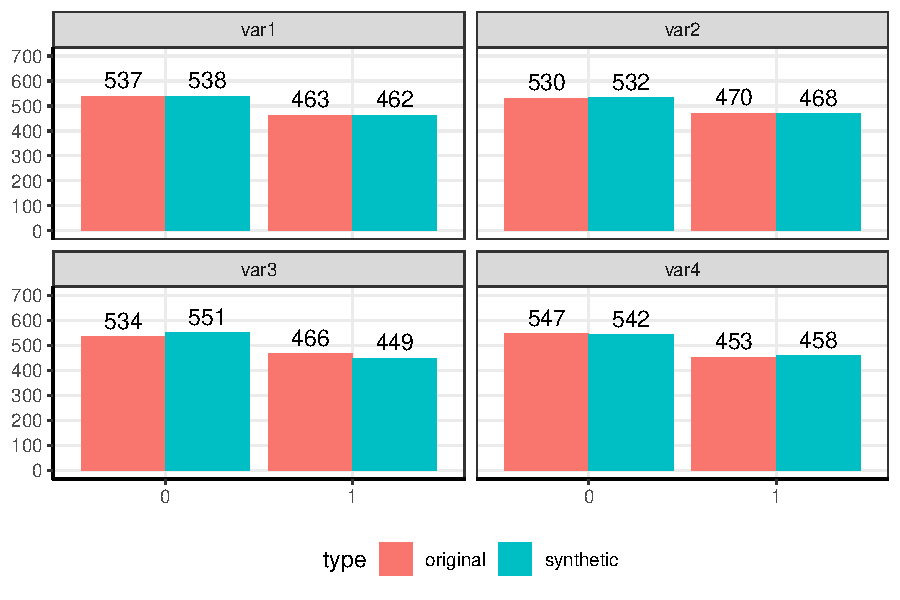
\includegraphics[width=\textwidth]{../../graphs/graph_cart_frequency_compare.pdf}
        \label{fig:frequency_compare}
    \end{figure}
\end{minipage}
\hfill
\begin{minipage}{0.48\textwidth}
    \begin{figure}
        \centering
        \caption{Histogram}
        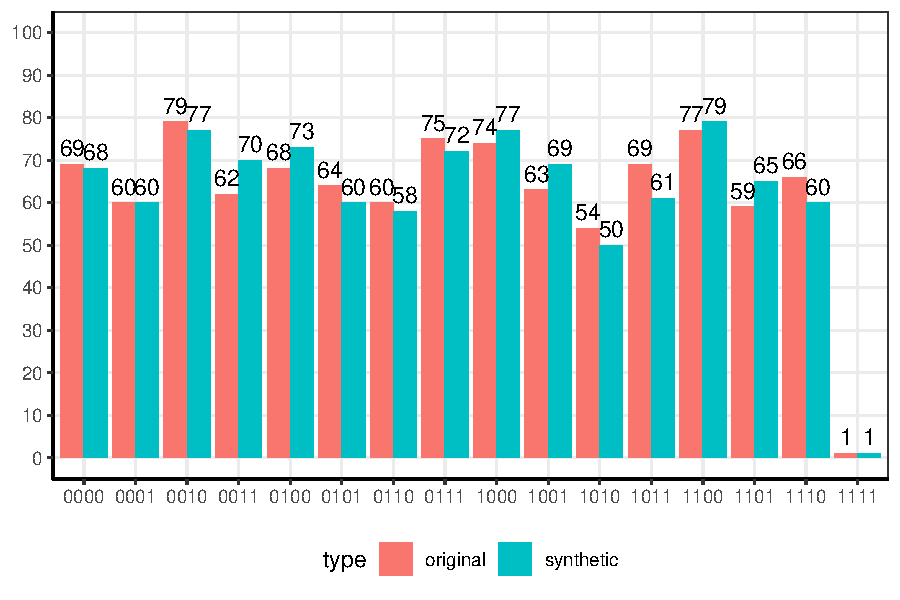
\includegraphics[width=\textwidth]{../../graphs/graph_cart_histogram_compare.pdf}
        \label{fig:histogram_compare}
    \end{figure}
\end{minipage}
\end{frame}

\begin{frame}[t]\frametitle{Compare histogram x 10 synthetic datasets}

\begin{figure}
    \caption{Multiple synthetic data sets does not reduce privacy risk}
    \resizebox{\textwidth}{!}{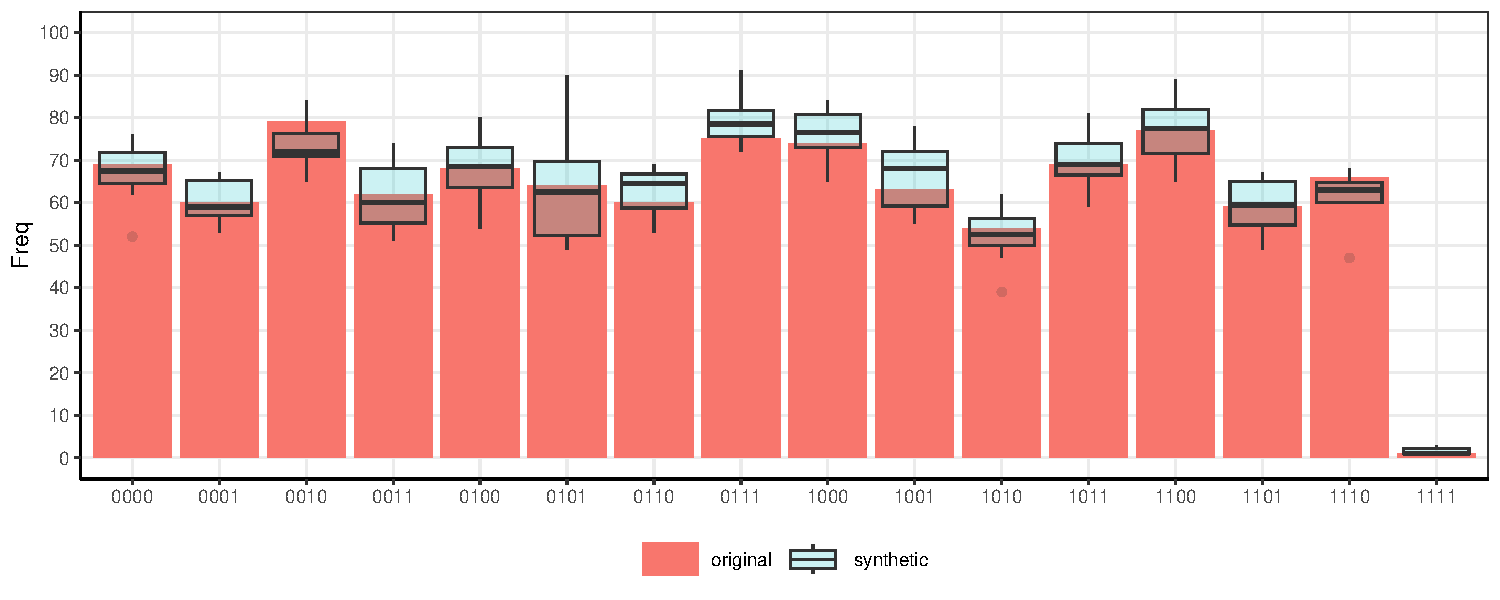
\includegraphics{../../graphs/graph_cart_histogram_compare_10_v1.pdf}}
    \label{fig:cart_histogram_compare_10}
\end{figure}

\end{frame}

\frame{\frametitle{Summary}
\begin{itemize}
    \item The problem (in our data): Synthetic data from CART models are disclosive
    \item The reason: 
    \begin{itemize}
        \item A record can only be in the synthetic data if it is also in the original data (in this simulated data).   
        \item Or the opposite: if a record is not in the original data, then it can never be in the synthetic data.
    \end{itemize}  
    \item Next section: Can an attacker identify the disclosure?
\end{itemize}
}

%%%%%%%%%%%%%%%%%%%%%%%%%%%%%%%%%%%%%%%%
%%%%%%%%%%%%%%%%%%%%%%%%%%%%%%%%%%%%%%%%
\section{The attack}\label{sec:attack}
%%%%%%%%%%%%%%%%%%%%%%%%%%%%%%%%%%%%%%%%
%%%%%%%%%%%%%%%%%%%%%%%%%%%%%%%%%%%%%%%%
\begin{frame}[c,plain]
\vskip-4mm
\begin{beamercolorbox}[wd=\boxwidth,ht=22.11mm]{transparent}%
    \vfill%
    \usebeamerfont{title}%
    \leftinsert%
    \MakeUppercase{Section \ref{sec:attack}: The attack
} % <- Hier die Überschrift eintragen
\end{beamercolorbox}
\vskip-3mm
\pgfuseimage{rahmenlinie}

\end{frame}

\frame{\frametitle{Describing the attack}
\begin{itemize}
    \item We assume a `strong' attacker similar to the attack model in differential privacy (DP). 
    \item An attacker has the following knowledge
    \begin{itemize}
        \item Knows the SDG model type (i.e. sequential CART).
        \item Knowledge of all observations in the data except the last one.  
        \item The 16 possible combinations that the last one could be.
    \end{itemize}
    \item The attacker sees the synthetic data
    \item The attacker runs the same synthetic data model (SDG) for all of the 16 different possibilities.  
    \item Then they update their beliefs about what the last record could be
\end{itemize}
}

\begin{frame}[t]\frametitle{Histogram of 16 worlds x 10 synthetic datasets}

\begin{figure}
    \caption{}
    \vskip -4mm
    \resizebox{\textwidth}{!}{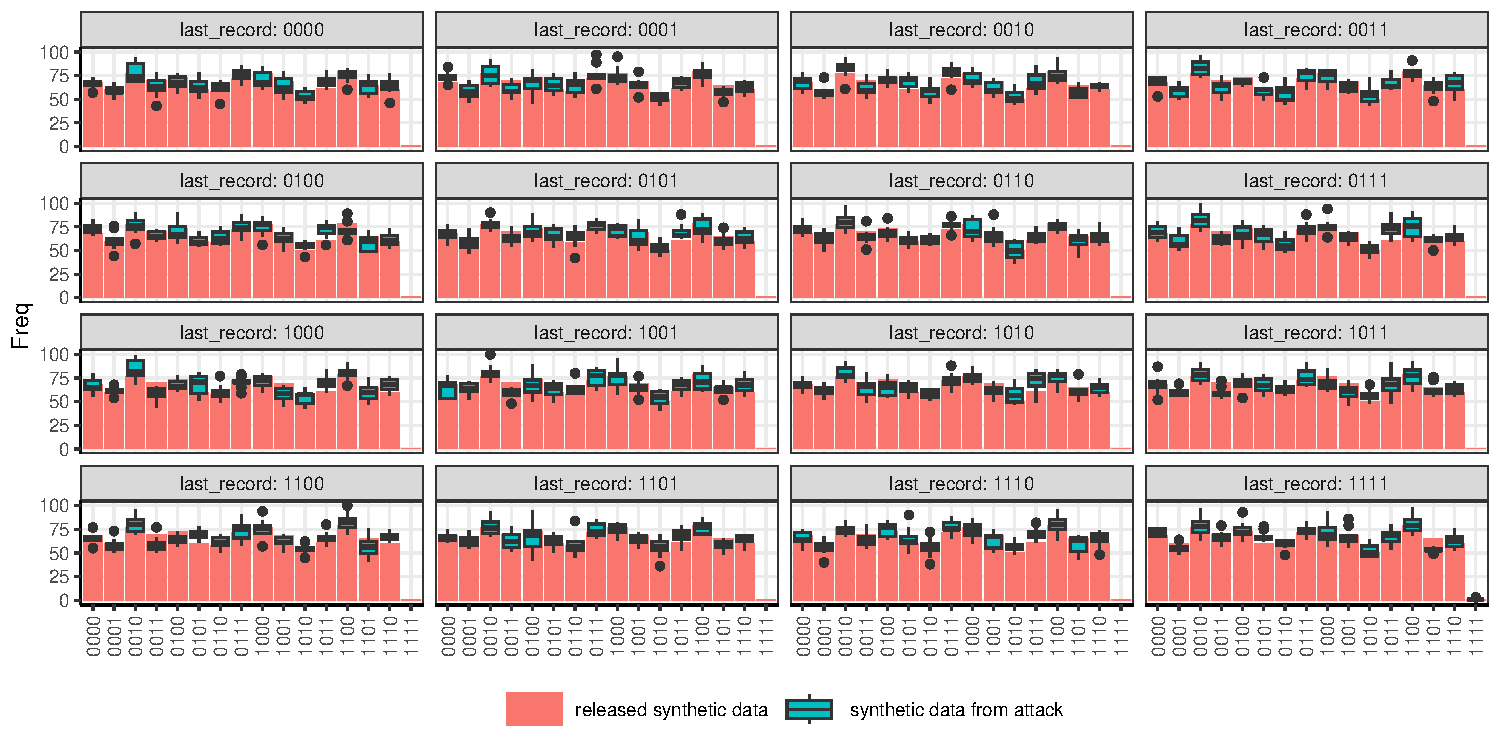
\includegraphics{../../graphs/graph_attacker_default_v1.pdf}}
    \label{fig:attacker_default}
\end{figure}


\end{frame}



\frame{\frametitle{Summary}
\begin{itemize}
    \item In our attack with our assumptions, the attacker can easily identify the last record
    \item The reason (to repeat): 
    \begin{itemize}
        \item A record can only be in the synthetic data if it is also in the original data (in this simulated data).   
        \item Or the opposite: if a record is not in the original data, then it can never be in the synthetic data.
    \end{itemize}  
    \item Next section: Can we measure this disclosure?
\end{itemize}

}


%%%%%%%%%%%%%%%%%%%%%%%%%%%%%%%%%%%%%%%%
%%%%%%%%%%%%%%%%%%%%%%%%%%%%%%%%%%%%%%%%
\section{Measuring disclosure risk}\label{sec:disclosure}
%%%%%%%%%%%%%%%%%%%%%%%%%%%%%%%%%%%%%%%%
%%%%%%%%%%%%%%%%%%%%%%%%%%%%%%%%%%%%%%%%
\begin{frame}[c,plain]
\vskip-4mm
\begin{beamercolorbox}[wd=\boxwidth,ht=22.11mm]{transparent}%
    \vfill%
    \usebeamerfont{title}%
    \leftinsert%
    \MakeUppercase{Section \ref{sec:disclosure}: Measuring disclosure risk
} % <- Hier die Überschrift eintragen
\end{beamercolorbox}
\vskip-3mm
\pgfuseimage{rahmenlinie}
\end{frame}

\begin{frame}[t]\frametitle{Disclosure risk measures}

\begin{itemize}
    \item The literature on privacy measures for synthetic data is well-developed (Wagner and Eckhoff, 2018).  
    \item Common privacy measures - Synthpop (Raab et al., 2025)
    \begin{itemize}
        \item Identity risk ($repU$): the ability to identify individuals in the data from a set of known characteristics or `keys' ($q$).  
        \item Attribute risk ($DiSCO$): the ability to find out from the keys something, not previously known or `target' ($t$)
    \end{itemize}
    \item Less common measures (Reiter et al., 2014)
    \begin{itemize}
        \item Bayesian risk: the probability that an intruder assigns to the true record after seeing the synthetic data.  
        \begin{itemize}
            \item If this probability is close to the prior (e.g. $1/K$ under a uniform prior), little information is revealed.  
            \item If it is much higher, the intruder has gained information; at $=1$, the record is identified with certainty.  
        \end{itemize}
    \end{itemize}
    \item In our data, we will show that attribute disclosure risk only indicates risk when there is no risk
\end{itemize}
\end{frame}

\begin{frame}[t]\frametitle{Identity risk}

$repU$ (replicated uniques) are unique records in the original data that are also unique in synthetic data and is the measure of identity risk.  Formally, $repU$ is defined by equation \ref{eq:repU}:

\begin{equation}
repU = 100 \sum (s_{.q}|d_{.q} = 1 \land s_{.q} = 1 )/N_{d}
\label{eq:repU}
\end{equation}

where $d_{.q}$ is the count of records in the original data with the keys corresponding to a given value of $q$ and $s_{.q}$ is the equivalent count for the synthetic data.  

In a given value of $q$, $s_{.q}|d_{.q} = 1$ is a unique record in the original data conditional on also existing in the synthetic data.  

AND

$s_{.q} = 1$ is the unique record in the synthetic data.  

This is summed over unique values of $q$ and divided by the total number of records in the data ($N_{d}$) and multiplied by 100 to transform the count into a percentage.


\end{frame}

\begin{frame}[t]\frametitle{Attribute risk}

$DiSCO$ (Disclosive in Synthetic Correct in Original) is the subset of records in the original data for which the keys ($q$) in the synthetic data is disclosive. $q$ is disclosive if all records in the synthetic data with the same $q$ have a constant target ($t$), i.e. no variation in $t$, as defined by the following equation \ref{eq:DiSCO}:

\begin{equation}
DiSCO = 100 \sum^{q} \sum^{t} (d_{tq} | ps_{tq} = 1) / N_{d}
\label{eq:DiSCO}
\end{equation}

where $d_{tq} | s_{tq} = 1$ indicates whether the synthetic data matches the original data for the combination of $t$ and $q$ given the condition that the synthetic data for the combination of $t$ and $q$ is disclosive (i.e., target $t$ is uniquely determined by the keys $q$).  

This is summed over unique values of $t$ and unique values of $q$ and divided by the total number of records in the data ($N_{d}$) and multiplied by 100 to transform the count into a percentage.
\end{frame}

\begin{frame}{Bayesian estimation of disclosure risk}
\begin{itemize}
    \item A Bayesian perspective asks: how much can an intruder learn about a specific record from the synthetic data? 
    \item The intruder is assumed to know all records except one, as well as the data synthesis algorithm.
    \item Using this information, the intruder combines prior beliefs with the released synthetic data to form a posterior distribution over the possible values of the unknown record.
    \item Disclosure risk is measured by the probability that the intruder assigns to the true record. 
    \begin{itemize}
        \item If this probability is close to the prior (e.g. $1/K$ under a uniform prior), then little information is revealed. 
        \item If the probability is much higher, the intruder has gained knowledge; in the extreme case the record could be identified with certainty.
    \end{itemize}
    \item We apply this measure to CART-based synthetic data generators in simple settings 
    \begin{itemize}
        \item (e.g. a dataset with four binary variables, where there are $K=16$ possible records).
    \end{itemize}
    \item In practice, this approach is rarely used because the number of possible records grows exponentially with the number of variables, making the calculations infeasible for large or complex datasets.
\end{itemize}
\end{frame}


\begin{frame}[t]\frametitle{Results disclosure risk measures}
\begin{minipage}[t]{0.48\textwidth}
    \begin{table}[]
        \centering
        \caption{x 1 synthetic data set (seed = 1237)}
        \resizebox{\textwidth}{!}{% latex table generated in R 4.5.0 by xtable 1.8-4 package
% Wed Aug 13 15:48:17 2025
\begin{tabular}{lrrrr}
  \toprule
Data & Unique &  Identity Risk  & Attribute Risk  & Bayesian Estimate of Risk \\ 
 & & ($repU$) & ($DiSCO$) & \\
  \midrule
Original & 1&  0.00 & 0.00 &  1.00 \\ 
  Synthetic & 1& 0.00 & 0.00 & 1.00 \\ 
   \bottomrule
\end{tabular}
}
        \label{table:disclosure_risk_1}
    \end{table}
\end{minipage}%
\hfill%
\begin{minipage}[t]{0.48\textwidth}
    \begin{table}[]
        \centering
        \caption{x 10 synthetic data sets}
        \rowcolors{1}{white}{lightgray}
        \resizebox{\textwidth}{!}{% latex table generated in R 4.5.0 by xtable 1.8-4 package
% Wed Aug 13 15:48:18 2025
\begin{tabular}{lrrr}
  \toprule
Data & Identity Risk ($repU$) & Attribute Risk ($DiSCO$) & Bayesian Estimate of Risk \\ 
  \midrule
Original & 0.00 & 0.00 & 1.00 \\ 
  Synthetic 1 & 0.00 & 0.00 & 1.00 \\ 
  Synthetic 2 & 0.00 & 6.60 & 0.02 \\ 
  Synthetic 3 & 0.00 & 0.00 & 1.00 \\ 
  Synthetic 4 & 0.00 & 0.00 & 1.00 \\ 
  Synthetic 5 & 0.00 & 0.00 & 1.00 \\ 
  Synthetic 6 & 0.00 & 0.00 & 1.00 \\ 
  Synthetic 7 & 0.00 & 0.00 & 1.00 \\ 
  Synthetic 8 & 0.00 & 6.60 & 0.03\\ 
  Synthetic 9 & 0.00 & 0.00 & 1.00 \\ 
  Synthetic 10 & 0.00 & 0.00 & 1.00 \\ 
  Average & 0.00 & 1.32 & - \\ 
   \bottomrule
\end{tabular}
}
        \label{table:disclosure_risk_10}
    \end{table}
\end{minipage}
\end{frame}



\frame{\frametitle{Summary}
\begin{itemize}
    \item Using common privacy measures, CART generates synthetic data with low risk
    \item However (and this is the point):
    \begin{itemize}
         \item We know there is a problem (because we created it)
         \item We know that common measures do not capture the problem 
    \end{itemize} 
    \item Further, $DiSCO$ only captures attribute risk when there is no attribute risk (i.e. no unique observation) 
\end{itemize}
}


%%%%%%%%%%%%%%%%%%%%%%%%%%%%%%%%%%%%%%%%
%%%%%%%%%%%%%%%%%%%%%%%%%%%%%%%%%%%%%%%%
\section{Is this scenario realistic?}\label{sec:reality}
%%%%%%%%%%%%%%%%%%%%%%%%%%%%%%%%%%%%%%%%
%%%%%%%%%%%%%%%%%%%%%%%%%%%%%%%%%%%%%%%%
\begin{frame}[c,plain]
\vskip-4mm
\begin{beamercolorbox}[wd=\boxwidth,ht=22.11mm]{transparent}%
    \vfill%
    \usebeamerfont{title}%
    \leftinsert%
    \MakeUppercase{Section \ref{sec:reality}: Is this scenario realistic?
} % <- Hier die Überschrift eintragen
\end{beamercolorbox}
\vskip-3mm
\pgfuseimage{rahmenlinie}

\end{frame}

\frame{\frametitle{Real world data (SD2011)}

Following the authors of Synthpop (Raab, 2024; Raab et al., 2024), we rely on data from Social Diagnosis 2011 (SD2011).  

In their paper, they generate 5 synthetic data sets to illustrate their method for measuring attribute disclosure by identifying values in the target variable \texttt{depress} from keys: \texttt{sex} \texttt{age} \texttt{region} \texttt{placesize}.  

To illustrate why it is a problem to measure attribute disclosure as the set of records with constant $t$ within $q$, we set $t$ as constant for all observations in all 5 synthetic data sets.  0 was chosen because it is the most frequent value in the variable \texttt{depress} (22\% of all records).  By definition, this reduces attribute disclosure risk.  

In their example, attribute risk is about 9\%. However, when we modify \texttt{depress} so that it is constant (0), the risk \emph{increased} to around 15\%.

Therefore, even though we know risk declined (because we reduced it), $DiSCO$ increases.

}

\begin{frame}[t]\frametitle{Results}

\begin{table}[!h]
    \centering
    \caption{Risk measures for \texttt{depress} from keys: \texttt{sex}, \texttt{age}, \texttt{region}, \texttt{placesize} (SD2011)}
    % \rowcolors{1}{white}{lightgray}
    % latex table generated in R 4.5.0 by xtable 1.8-4 package
% Fri Sep 19 10:19:15 2025
\begin{tabular}{lrrrr}
   
\toprule & 
\multicolumn{2}{l}{Identity risk ($repU$)} &
\multicolumn{2}{l}{Attribute risk ($DiSCO$)}
\\  
 
\cmidrule(lr){2-3}
\cmidrule(lr){4-5}
 
Data & Raab et al., 2024 & Modified & Raab et al., 2024 & Modified
\\ 

\midrule
Original data & 48.38 & 48.38 & 53.30 & 53.30 \\ 
   \midrule
Synthetic 1 & 14.82 & 14.82 & 8.96 & 14.74 \\ 
  Synthetic 2 & 14.20 & 14.20 & 9.90 & 14.82 \\ 
  Synthetic 3 & 15.16 & 15.16 & 10.46 & 14.94 \\ 
  Synthetic 4 & 14.12 & 14.12 & 9.68 & 14.50 \\ 
  Synthetic 5 & 14.30 & 14.30 & 8.88 & 14.66 \\ 
   \midrule
Average & 14.52 & 14.52 & 9.58 & 14.73 \\ 
   \bottomrule \\[-1.8ex] \multicolumn{5}{p{4in}}{Note: Modified indicates that values of \texttt{depress}=0 for all records in the synthetic data} 
\end{tabular}

    \label{tab:attribute_risk_sd2011}
\end{table}



\end{frame}

\frame{\frametitle{Identifying disclosure from 1-way}

The package authors are aware that the $DiSCO$ measure of attribute disclosure risk can indicate a high level of risk for a target variable where a high proportion of records have one level (Raab et al., 2024).

The package includes a flag to allow the user to identify values within a variable that explain most of the disclosures (\texttt{check\_1way}).

The authors give an example where the target variable is \texttt{workab}, where 89\% of the observations never worked abroad.  

The authors suggest that this level of $t$ for a group with the same $q$ would not be disclosive.

We agree, but our example illustrates that the disclosure measure increases, when it should decrease.


}

\frame{\frametitle{Summary}
\begin{itemize}
    \item When we create synthetic data to reduces attribute disclosure risk, $DiSCO$ measure increases
    \item The key point is that we show that $DiSCO$ mismeasures risk using real world data
\end{itemize}
}


%%%%%%%%%%%%%%%%%%%%%%%%%%%%%%%%%%%%%%%%
%%%%%%%%%%%%%%%%%%%%%%%%%%%%%%%%%%%%%%%%
\section{Conclusion}\label{sec:conclusion}
%%%%%%%%%%%%%%%%%%%%%%%%%%%%%%%%%%%%%%%%
%%%%%%%%%%%%%%%%%%%%%%%%%%%%%%%%%%%%%%%%
\begin{frame}[c,plain]
\vskip-4mm
\begin{beamercolorbox}[wd=\boxwidth,ht=22.11mm]{transparent}%
    \vfill%
    \usebeamerfont{title}%
    \leftinsert%
    \MakeUppercase{Section \ref{sec:conclusion}: Conclusion} % <- Hier die Überschrift eintragen
\end{beamercolorbox}
\vskip-3mm
\pgfuseimage{rahmenlinie}
\end{frame}

\frame{\frametitle{Summary}
\begin{itemize}
    \item It has long been understood that there is a trade-off between utility and risk
    \item Previous research indicated that CART models were less sensitive to this trade-off than other SDGs 
    \item Using a simulated data set, we show that CART are sensitive to this trade-off
    \item The good news: It is possible to reduce risk in CART with parameters
    \item The bad news: Common privacy metrics do not capture risk
    \begin{itemize}
        \item $DiSCO$ indicates risk when there is no risk (simulation)
        \item $DiSCO$ indicates risk increases when we know it decreased (SD2011)
    \end{itemize}
\end{itemize}
}

\frame{\frametitle{Thank you}

Jonathan Latner: \url{jonathan.latner@iab.de} \\

Reproducible code: \url{https://github.com/jonlatner/KEM\_GAN/tree/main/latner/projects/simulation} 

}



\end{spacing}
\end{document}

